\documentclass[12pt,openright,twoside,a4paper,english,french,spanish]{abntex2}

% ---
% PACOTES
% ---

% ---
% Pacotes fundamentais 
% ---
\usepackage{cmap}				% Mapear caracteres especiais no PDF
\usepackage{lmodern}			% Usa a fonte Latin Modern			
\usepackage[T1]{fontenc}		% Seleção de códigos de fonte.
\usepackage[utf8]{inputenc}		% Determina a codificação utiizada (conversão automática dos acentos)
\usepackage{makeidx}            % Cria o indice
\usepackage{hyperref}  			% Controla a formação do índice
\usepackage{lastpage}			% Usado pela Ficha catalográfica
\usepackage{indentfirst}		% Indenta o primeiro parágrafo de cada seção.
\usepackage{color}				% Controle das cores
\usepackage{graphicx}			% Inclusão de gráficos
% ---

% ---
% Pacotes adicionais, usados apenas no âmbito do Modelo Canônico do abnteX2
% ---
\usepackage{lipsum}				% para geração de dummy text
% ---

% ---
% Pacotes de citações
% ---
\usepackage[brazilian,hyperpageref]{backref}	 % Paginas com as citações na bibl
\usepackage[alf]{abntex2cite}	% Citações padrão ABNT


%\usepackage[nonumberlist,style=altlist]{glossaries}	% Glossario
\usepackage[brazil]{translator}
\usepackage[
nonumberlist, %do not show page numbers
acronym,      %generate acronym listing
numberline,
toc]      %use section level for toc entries
{glossaries}


% Listings (código-fonte)
\usepackage{listings}
\usepackage{color}
\usepackage[usenames,dvipsnames]{xcolor}
\usepackage{caption}

% Estilo do caption dos algoritmos
\DeclareCaptionFont{white}{\color{white}}
\DeclareCaptionFormat{listing}{\colorbox{gray}{\parbox{\textwidth}{#1#2#3}}}
\captionsetup[lstlisting]{format=listing,labelfont=white,textfont=white}

\definecolor{sourceCodeBG}{rgb}{0.95,0.95,0.95}

\renewcommand*{\lstlistlistingname}{Lista de Algoritmos}
\renewcommand*{\lstlistingname}{Algoritmo}




\lstnewenvironment{sourcecode}[2]
{\lstset{
		language = [Objective]C,
        numbers = left,
		showspaces=false,
		showstringspaces=false,
        numberstyle = \footnotesize,
        tabsize = 2,
        frame = none,
        captionpos = tb,
		basicstyle=\ttfamily,
		breaklines=true,
		% Colors
		backgroundcolor=\color{sourceCodeBG},
		keywordstyle=\color{BlueViolet},          % keyword style
		identifierstyle=\color{black},
		commentstyle=\color{OliveGreen},       % comment style
		stringstyle=\color{red},         % string literal style
		%numberstyle=\color{blue},
		% Adiciona novas palavras-chave e diretivas
		morekeywords={@catch,@class,@encode,@end,@finally,@implementation,%
		      @interface,@private,@protected,@protocol,@public,@selector,%
		      @synchronized,@throw,@try,BOOL,Class,IMP,NO,Nil,SEL,YES,_cmd,%
		      bycopy,byref,id,in,inout,nil,oneway,out,self,super,%
		      @dynamic,@package,@property,@synthesize,readwrite,readonly,%
		      assign,retain,copy,nonatomic, @required, @optional%
		      },
		moredirectives={import},
 		% Atribui o label e o caption, passados por parâmetro
		label = #1,
        caption = #2
        }
}
{}





\makeglossaries
%%%%%%%%%%%%%%%%%%%%%%%%%%%%%%%%%%%%%
% Siglas
%%%%%%%%%%%%%%%%%%%%%%%%%%%%%%%%%%%%%
% Padrão:
%\newacronym{LABEL}{NOME}{DESC}
% ou ligado ao glossário:
%\newacronym{LABEL}{NOME}{DESC\protect\glsadd{glos:LABEL}}



\newacronym{API}{API}{Application Programing Interface}
\newacronym{WS}{WS}{WEB Service\protect\glsadd{glosWS}}
\newacronym{6DOF}{6DoF}{Six Degrees of Freedom\protect\glsadd{glos6DOF}}
\newacronym{XML}{XML}{Extensible Markup Language\protect\glsadd{glosXML}}
\newacronym{JSON}{JSON}{JavaScript Object Notation\protect\glsadd{glosJSON}}
\newacronym{HMD}{HMD}{Head Mounted Display\protect\glsadd{glosHMD}}
\newacronym{GPS}{GPS}{Global Positioning System\protect\glsadd{glosGPS}}
\newacronym{SGBD}{SGBD}{Sistema Gerenciador de Banco de Dados}
\newacronym{SDK}{SDK}{Software Development Kit\protect\glsadd{glosSDK}}




%%%%%%%%%%%%%%%%%%%%%%%%%%%%%%%%%%%%%%
% Termos do Glossário
%%%%%%%%%%%%%%%%%%%%%%%%%%%%%%%%%%%%%%
% Padrão:
% \newglossaryentry{glos:<LABEL>}{
%name=<NOME>,
%description={<DESC>}
%}


\newglossaryentry{glos5R_Adapt_Rules}{
name=5R das Regras de Adaptação (\textit{5R Adaption Rules}),
description={Conteúdo adequado, na hora certa, no lugar correto, no dispositivo adequado para as pessoas certas (\textit{\textbf{R}ight Contents on the \textbf{R}ight Time at \textbf{R}ight Place to \textbf{R}ight Device for \textbf{R}ight People})}
}

\newglossaryentry{glos6DOF}{
name=6 Graus de Liberdade (\textit{Six Degrees of Freedom}),
description={O 6DoF se refere ao livre movimento de um corpo no espaçco tridimensional. Ou seja, o corpo pode se mover para cima/baixo, diretia/esquerda e para frente/trás. Além disso, ele pode se rotacionar pelos três eixos perpendiculares. Veja mais detalhes na Seção \ref{sec:vision-based-tracking}, página \pageref{sec:vision-based-tracking} e na Figura \ref{fig:6dof_data}}
}



\newglossaryentry{glosWS}{
name=Web Service,
description={É uma solução utilizada na integração de sistemas e na comunicação entre aplicações diferentes. Com esta tecnologia é possível que novas aplicações possam interagir com aquelas que já existem, e que sistemas desenvolvidos em plataformas diferentes sejam compatíveis. Essa integração é possível devido ao envio e recebimento de dados em formato XML.}
}


\newglossaryentry{glosXML}{
name=Extensible Markup Language (XML),
description={É uma recomendação da W3C para gerar linguagens de marcação para necessidades especiais. Seu propósito principal é a facilidade de compartilhamento de informações através da internet. Descrita no RFC 3023}
}


\newglossaryentry{glosJSON}{
name=JavaScript Object Notation (JSON),
description={É uma notação aplicada em JavaScript para que se possa definir de forma clara objetos de estruturas complexas. O formato JSON é descrito no RFC 4627.}
}


\newglossaryentry{glosHMD}{
name=Head Mounted Display,
description={É um dispositivo semelhante um capacete, que possui uma tela pela qual o usuário visualiza imagens provenientes de um computador. Veja definição completa na Seção \ref{sec:ra_mobile}, página \pageref{def:hmd} e a imagem ilustrativa na Figura \ref{fig:hmd_example}}
}


\newglossaryentry{glosGPS}{
name=Global Positioning System,
description={Sistema de navegação por satélite que fornece a um aparelho receptor móvel a sua posição na Terra, a qualquer momento e em qualquer lugar, desde que este se encontre no campo de visão de, pelo menos, quatro satélites GPS}
}


\newglossaryentry{glosSDK}{
name=Software Development Kit,
description={em português, Kit de Desenvolvimento de Software ou Kit de de Desenvolvimento de Aplicativos. É um conjunto de ferramentas que permite a criação de apicações para determinado pacote de software, plataforma de hardware, sistema operacional etc.}
}












% Configurações do pacote backref
% Usado sem a opção hyperpageref de backref
\renewcommand{\backrefpagesname}{Citado na(s) página(s):~}
% Texto padrão antes do número das páginas
\renewcommand{\backref}{}
% Define os textos da citação
\renewcommand*{\backrefalt}[4]{
	\ifcase #1 %
		Nenhuma citação no texto.%
	\or
		Citado na página #2.%
	\else
		Citado #1 vezes nas páginas #2.%
	\fi}%
% ---




% ---
% Informações de dados para CAPA e FOLHA DE ROSTO
% ---
\titulo{Implementação de uma Aplicação Baseada em Realidade Aumentada para Geolocalização em um Campus Universitário}
\autor{Roberto Beraldo Chaiben}
\local{Curitiba}
\data{2012}
\orientador{Marcos Didonet Del Fabro}
\instituicao{Universidade Federal do Paraná -- UFPR}
%\tipotrabalho{Tese (Doutorado)}
% O preambulo deve conter o tipo do trabalho, o objetivo, 
% o nome da instituição e a área de concentração 
\preambulo{Trabalho de Conclusão de Curso apresentado ao Curso de Bacharelado em Ciência da Computação, do Departamento de Informática, Setor de Ciências Exatas, Universidade Federal do Paraná}
% ---



% ---
% Configurações de aparência do PDF final

% alterando o aspecto da cor azul
\definecolor{blue}{RGB}{41,5,195}

% informações do PDF
\hypersetup{
     	%pagebackref=true,
		pdftitle={\imprimirtitulo}, 
		pdfauthor={\imprimirautor},
    	pdfsubject={\imprimirpreambulo},
		pdfkeywords={PALAVRAS}{CHAVES}{abnt}{abntex}{abntex2},
	    pdfproducer={LaTeX with abnTeX2}, 	% producer of the document
	    pdfcreator={\imprimirautor},
    	colorlinks=true,       		% false: boxed links; true: colored links
    	linkcolor=blue,          	% color of internal links
    	citecolor=blue,        		% color of links to bibliography
    	filecolor=magenta,      		% color of file links
		urlcolor=blue,
		bookmarksdepth=4
}
% --- 

% --- 
% Espaçamentos entre linhas e parágrafos 
% --- 

% O tamanho do parágrafo é dado por:
\setlength{\parindent}{1.3cm}

% Controle do espaçamento entre um parágrafo e outro:
\setlength{\parskip}{0.2cm}  % tente também \onelineskip

% ---
% compila o indice
% ---
\makeindex
% ---






\begin{document}


% Retira espaço extra obsoleto entre as frases.
\frenchspacing 

% ----------------------------------------------------------
% ELEMENTOS PRÉ-TEXTUAIS
% ----------------------------------------------------------
% \pretextual

% ---
% Capa
% ---
\imprimircapa
% ---

% ---
% Folha de rosto
% (o * indica que haverá a ficha bibliográfica)
% ---
\imprimirfolhaderosto*
% ---

% ---
% Inserir a ficha bibliografica
% ---





% ---
% Epígrafe
% ---
\begin{epigrafe}
    \vspace*{\fill}
	\begin{flushright}
		\textit{"I don't believe that the ultimate theory will come by steady work along existing lines. We need something new. We can't predict what that will be or when we will find it because if we knew that, we would have found it already!." \\Stephen Hawking}
	\end{flushright}
\end{epigrafe}
% ---

% ---
% RESUMOS
% ---

% resumo em português
\begin{resumo}
    A Realidade Aumentada, uma área derivada da Realidade Virtual e que vem 
    ganhando espaço nos últimos 20 anos.  A Realidade Aumentada permite 
    criar objetos virtuais sobrepostos à realidade vista pelos usuários, com 
    auxílio de técnicas de Visão Computacional. A Realidade Aumentada também permite a 
    interação dos usuários com esses objetos virtuais, o que cria um ambiente 
    interativo de aprendizado. 
    Este trabalho tem como objetivo implementar  um 
    aplicativo para dispositivos móveis, baseado em Realidade Aumentada, para auxílio 
    na geolocalização de usuários em um campus universitário.

 \vspace{\onelineskip}
    
 \noindent
 \textbf{Palavras-chaves}: Realidade Aumentada, Realidade Virtual, Geolocalização, Tracking, Registration.
\end{resumo}


% resumo em inglês
\begin{resumo}[Abstract]
 \begin{otherlanguage*}{english}
    Augmented Reality is an area derived from Virtual Reality, which
    has been growing in the last 20 years. Augmented Reality allows us to create
    overlaid virtual objects on the reality seen by the user, using
    Computer Vision techniques. Augmented Reality allows the interaction of the users
    with the virtual objects, which creates an interative learning environment. 
    This work aims to develop a university campus geolocation application, based on Augmented Reality.
    



   \vspace{\onelineskip}
 
   \noindent 
   \textbf{Key-words}: Augmented Reality, Virtual Reality, Geolocation, Tracking, Registration.
 \end{otherlanguage*}
\end{resumo}







% ---
% inserir lista de ilustrações
% ---
\pdfbookmark[0]{\listfigurename}{lof}
\listoffigures
\cleardoublepage
% ---

% ---
% inserir lista de tabelas
% ---
\pdfbookmark[0]{\listtablename}{lot}
\listoftables
\cleardoublepage
% ---


% ---
% inserir lista de Algoritmos
% ---
\pdfbookmark[0]{\listtablename}{lot}
\lstlistoflistings
\cleardoublepage
% ---


% Glossário
\pdfbookmark[0]{\listtablename}{lot}
%\newpage
\glsaddall

%Traduções para o ambiente glossaries
\providetranslation{Glossary}{Glossário}
\providetranslation{Acronyms}{Siglas}
\providetranslation{Notation (glossaries)}{Notação}
\providetranslation{Description (glossaries)}{Descrição} 
\providetranslation{Symbol (glossaries)}{Síimbolo}
\providetranslation{Page List (glossaries)}{Lista de Páginas} 
\providetranslation{Symbols (glossaries)}{Símbolos}
\providetranslation{Numbers (glossaries)}{Números}

\glossarystyle{altlisthypergroup}
\printglossaries
\cleardoublepage



% ---
% inserir o sumario
% ---
\pdfbookmark[0]{\contentsname}{toc}
\tableofcontents*
\cleardoublepage
% ---







% ----------------------------------------------------------
% ELEMENTOS TEXTUAIS
% ----------------------------------------------------------
% É possível usar \textual ou \mainmatter, que é a macro padrão do memoir.  
\mainmatter





%====================================================

\chapter{Introdução}


A Realidade Aumentada (\textit{Augmented Reality})
é um ramo da Realidade Virtual 
que vem sendo estudado nos últimos anos. Essa tecnologia
mescla os últimos avanços no Processamento de Imagens Digitais,
Inteligência Artificial, sensores de GPS, reconhecimento e
técnicas de interação humano-computador. Ela é largamente utilizada
em entretenimento, pesquisas científicas e militares, Medicina, manufatura e manutenção
de máquinas e muitas outras áreas \cite{ARFeatureMaching, DevActuallyRegistration}.

A Realidade Aumentada consiste na sobreposição de objetos virtuais, gerados por
computação, a imagens do mundo real, geralmente capturadas por câmeras digitais. Esse é
um processo em tempo real, como a exibição do placar na televisão durante uma partida
de futebol. 

Com a ajuda de técnicas avançadas de Realidade Aumentada, como visão computacional,
reconhecimento de objetos e geolocalização, as informações acerca da realidade que envolve o usuário
tornam-se interativas e digitalmente manipuláveis. Esses dados podem ser sobrepostos
às imagens que o usuário visualiza por meio de algum dispositivo de saída, como a tela de um
\textit{smartphone} ou \textit{tablet} \cite{AReX}.


A primeira interface usando Realidade Aumentada foi criada por Ivan Edward Sutherland, na década de 1960. 
Apesar disso, a primeira conferência especialmente dedicada a esse tema foi realizada apenas 
em 1998, o IWAR 98\footnote{International Workshop on Augmented Reality} \cite{TrendsInAR}. 
Sutherland, com ajuda de seu estudante Bob Sproull, criou o que foi considerado o primeiro dispositivo
de Ralidade Aumentada e Realidade Virtual. Esse instrumento consistia no que é chamado de \gls{HMD}, uma
espécie de capacete, onde há uma tela acoplada, por meio da qual o usuário visualiza imagens geradas
por um computador. Esse projeto foi chamado de \textit{The Sword of Damocles} \cite{TheUltimateDisplay}.


Dispositivos móveis vêm ganhando muito espaço nos últimos anos, como pode ser visto segundo a 
pesquisa da \textit{Strategy Analytics}
\footnote{\href{http://www.strategyanalytics.com}{http://www.strategyanalytics.com}}. A pesquisa revelou que,
em outubro de 2012, já existiam mais de 1 bilhão de dispositivos móveis e que em até 3 anos será ultrapassada 
a marca de 2 bilhões. 

Dispositivos como \textit{smartphones} e \textit{tablets} vêm ganhando cada vez mais funcionalidades, com 
melhorias de \textit{hardwares}. Esses equipamentos podem ser utilizados para tarefas diversas e uma das
principais é a geolocalização, uma vez que recursos de localização, como \gls{GPS} e bússola, equipam a 
maioria desses aparelhos.

As principais soluções de geolocalização atuais, como o Google Maps, utilizam mapas 2D. Esse tipo de 
disposição de dados pode ser muito bom para navegação em grandes territórios. Porém, para locais mais
específicos, deveria haver uma aplicação mais próxima à realidade do usuário, por meio da qual fosse 
possível visualizar não apenas um mapa 2D da área onde ele está, mas, também, exibir as construções 
à sua volta, explicitando na tela do dispositivo a direção de cada ponto de interesse, bem como a distância
até eles.

Este trabalho descreve uma solução para esse problema. O objetivo é implementar um aplicativo, baseado em 
Realidade Aumentada, para geolocalização em 
um campus universitário. A solução desenvolvida utiliza a Realidade Aumentada para orientar o
usuário no Centro Politécnico da Universidade Federal do Paraná. A partir das coordenadas geográficas de alguns 
pontos de interesse, como blocos de salas de aula, departamentos e secretarias de cursos e Restaurante Universitário, 
a aplicação cria duas interfaces principais: um mapa 2D, onde cada ponto é identificado por um marcador, como na maioria
dos aplicativos de geolocalização; a outra interface utiliza a Realidade Aumentada. Ela exibe as imagens capturadas pela
câmera do dispositivo, sobrepostas com as identificações dos pontos de interesse do usuário. Conforme o usuário move o
equipamento, esses marcadores se movem na tela, orientando o usuário para qual direção cada ponto está, além da distância
até eles. A aplicação também permite cadastrar locais de interesse próprios do usuário, não restringindo o uso apenas com os
pontos de interesse fornecidos pelo sistema.











\chapter{Realidade Aumentada}
\label{chapter:principios_ra}



A Realidade Aumentada aprimora a percepção do mundo pelo usuário, além de
lhe permitir interagir com essa realidade. Os objetos virtuais podem 
exibir informações que os usuários não detectariam diretamente sozinhos.
Esses dados podem ajudar os usuários a realizar tarefas reais do dia-a-dia
\cite{SurveyAR}.


Um dos principais pesquisadores sobre Realidade Aumentada nos últimos 20 anos
é o Ronald T. Azuma. Segundo ele, toda aplicação de Realidade Aumentada deve possuir
as seguintes características \cite{SurveyAR}:


% Azuma não detalha estes tópicos, por isso não foram melhores descritos aqui
\begin{enumerate}
    \item Combinação dos mundos real e virtual
    \item Interatividade em tempo real
    \item Sobreposição de objetos virtuais em 3D
\end{enumerate}







\section{Realidade Virtual e Realidade Aumentada}

A Realidade Aumentada é uma área derivada da Realidade Virtual, com distinções,
vantagens e desvantagens para determinados tipos de aplicações. Nas subseções 
seguintes serão abordadas essas características.


\subsection{Realidade Virtual}


A Realidade Virtual é uma técnica que viabiliza a interação de elementos reais em ambientes
virtuais, gerados por computação. 
Um bom exemplo de Realidade Virtual são os simuladores de voo, simuladores de corrida etc, usados
por muitos pilotos durante treinamento e preparação.
Dessa forma, a Realidade Virtual é a completa imersão do usuário em um ambiente totalmente
gerado computacionalmente. A interação do usuário com esse ambiente é feita por meio de capacetes,
luvas ou outros equipamentos que permitam a transmissão de informações de movimentos e ações 
do usuário ao computador \cite{ARColaborativa}.

Diversas aplicações, como tratamento de doenças e fobias, simulação de exames
médicos e procedimentos cirúrgicos, além de técnicas de extração de petróleo
podem ser beneficiadas com o uso da Realidade Virtual \cite{ARColaborativa}.


A Figura \ref{fig:equipamentos_rv} exibe alguns exemplos de equipamentos utilizados na Realidade
Virtual, para permitir a interação do usuário com a realidade gerada pela aplicação.

\begin{figure}[h!]
    \centering
    \caption{Exemplo de Equipamentos utilizados na Realidade Virtual}
    \label{fig:equipamentos_rv}
    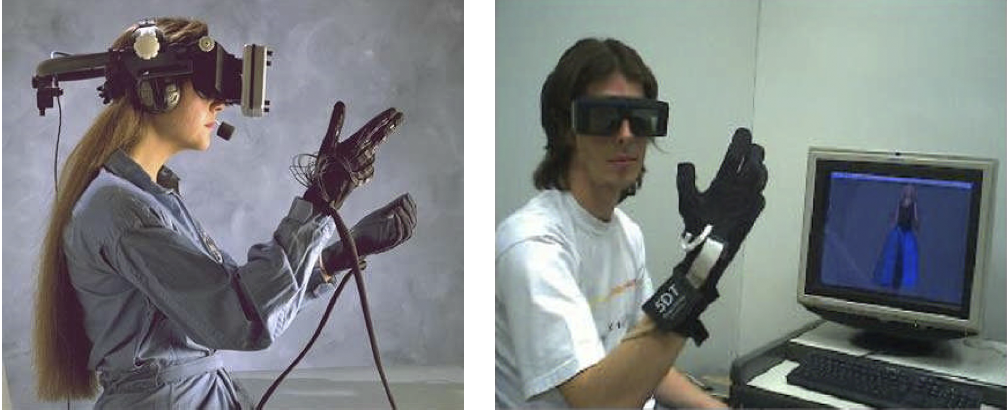
\includegraphics[width=14cm]{resources/equipamentos-rv.png}
\end{figure}



\subsection{Realidade Aumentada}


A Realidade Aumentada consiste na sobreposição de informações (imagens, textos e outros dados) a imagens
do mundo real, geralmente obtidas a partir de câmeras. Muitas aplicações estão usando a Realidade Aumentada
para prover maior interação entre o usuário e as informações ao seu redor. Um exemplo de aplicação da 
Realidade Aumentada é a sobreposição do fluxo sanguíneo em uma imagem dos vasos sanguíneos de um paciente,
obtida a partir de um exame médico \cite{ARColaborativa}.

A Figura \ref{fig:AR-map-locations11} mostra um exemplo de aplicação de Realidade Aumentada para geolocalização.

\begin{figure}[h!]
    \centering
    \caption{Exemplo de Realidade Aumentada para localização}
    \label{fig:AR-map-locations11}
    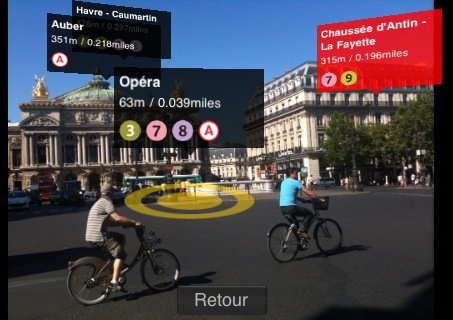
\includegraphics[width=15cm]{resources/augmented-reality-paris.jpg}
\end{figure}



\subsection{Diferenças entre Realidade Virtual e Realidade Aumentada}

A principal diferença entre Realidade Virtual e Realidade Aumentada
é que a primeira cria uma nova realidade ao usuário, com objetos
próprios, todos criados pela computação. Já a Realidade Aumentada
sobrepõe objetos virtuais a imagens da realidade humana, geralmente
captadas por câmeras digitais \cite{ARCADE, TrendsInAR}.
Segundo \cite{SurveyAR, AdvancesAR}, a Realidade Aumentada é
um suplemento à realidade, não uma substituição dela, de forma que,
para o usuário, a realidade e os objetos virtuais coexistem no mesmo
espaço. A Realidade Aumentada exige muita precisão na detecção da
localização e da posição do usuário, para que seja possível fornecer
uma interface com o usuário poderosa, por exemplo, mostrando objetos
virtuais baseados na posição e na direção para onde o usuário está
voltado.

Em determinados tipo de aplicação, a Realidade Aumentada pode prover maiores vantagens em 
relação à Realidade Virtual, dentre elas \cite{ARFeatureMaching}:

\begin{itemize}
    \item \textbf{A Realidade Aumentada provê melhor senso de realidade}\\
    
    A Realidade Virtual simula o mundo real por meio da computação, dando a
    sensação de imersão ao usuário. Por outro lado, a Realidade Aumentada 
    é uma integração do mundo real com o ambiente virtual, o que dá mais senso
    de realidade aos usuários.
    
    \item \textbf{A Realidade Aumentada permite maior interatividade}\\
    
    Como a Realidade Virtual enfatiza o mundo virtual como sendo seu principal
    recurso, o usuário permanece em situação passiva. Contudo, a Realidade Aumentada
    considera fundamental a integração entre mundo real e objetos virtuais. Assim,
    a Realidade Aumentada permite que os usuários participem e interajam com ela.
\end{itemize}

A Tabela \ref{tab:dif_AR_VR} mostra as principais diferenças entre
Realidade Virtual e Realidade Aumentada.

\begin{table}[h!]
    \centering
    \caption{Principais Diferenças entre Realidade Virtual e Realidade Aumentada}
    \label{tab:dif_AR_VR}
    \begin{tabular}{| p{5cm} | p{5cm} | p{5cm} |}
         \hline
         & Realidade Virtual & Realidade Aumentada \\
         \hline
         Ambiente Principal & Gerado por computador & Mundo real \\
         \hline
         Sentido da Presença & Controlado por computador & Natural do usuário \\
         \hline
         Impacto da transição do mundo real para o virtual & Alta & Baixa \\
         \hline
         Representação do usuário & Através de um avatar & Direta \\
         \hline
    \end{tabular}
\end{table}

Pesquisas anteriores por \cite{AppsHandheldDevices} e \cite{FieldTrips}
concluíram que a combinação de detecção de localização do usuário e
abordagem de aprendizado contextual pode facilitar a construção de 
conceitos mais precisos por usuários dessas tecnologias.

O foco principal deste trabalho é a Realidade Aumentada, por ser mais adequada 
à aplicação proposta. Por se tratar de uma aplicação de geolocalização, o usuário
não pode ter a sensação de imersão em uma realidade criada computacionalmente. É
imprescindível que a realidade do usuário não seja alterada, apenas complementada 
com informações relevantes.






\section{Realidade Aumentada em Dispositivos Móveis}
\label{sec:ra_mobile}

O uso de dispositivos móveis vem aumentando muito rapidamente nos últimos anos.
Segundo a \textit{Strategy Analytics}
\footnote{\href{http://www.strategyanalytics.com}{http://www.strategyanalytics.com}},
em outubro de 2012, a quantidade de \textit{smartphones} no mundo ultrapassou a faixa
de 1 bilhão. Desse total, apenas no período entre setembro de 2011 a outubro de 2012, 
a soma foi de 330 milhões de novos dipositivos e 79 milhões no segundo quadrimestre de 2012.
Segundo essa mesma pesquisa, nos próximos 3 anos será atingida a marca de 2 bilhões de
\textit{smartphones}.


Até recentemente, a Realidade Aumentada era utilizada predominantemente 
em \textit{desktops} e em ambientes virtuais. Porém, \cite{SurveyAR}
considerou que um sistema de Realidade Aumentada ideal deveria 
funcionar em qualquer ambiente natural, sem limitação de alcance e sem prévio
conhecimento do local onde o sistema atuará.

A Realidade Aumentada Móvel (\textit{Mobile Augmented Reality}) foi criada e estudada
antes mesmo da criação dos dispositivos móveis atuais, como \textit{smartphones} e 
\textit{tablets} \cite{ExperiencesWithHandheldAR, HouseOfOlbrich}. Os pesquisadores acoplavam câmeras a
telas de computadores reduzidos, que possuíam um dispositivo de saída (\textit{display}),
onde eram exibidas as imagens para o usuário, após serem processadas pelo programa. 
Todo esse processo deveria ocorrer em tempo real, de forma a permitir ao usuário a interação
com o ambiente.



Os usuários de dispositivos móveis os utilizam para diversos objetivos, não somente para fazer
ligações, navegar na Internet ou verificar suas caixas de email. Uma das principais utilidades
dos \textit{smartphones} é para localização, via \gls{GPS}. Há muitas aplicações de mapas, 
com imagens provenientes 
de satélites etc, que facilitam a vida dos usuários, principalmente em viagens para locais não
conhecidos. Seguindo a mesma ideia de localização, é possível criar aplicações específicas para
esse fim, focadas em áreas menores e mais específicas, auxiliando o usuário a se localizar, por exemplo, dentro
de um campus de um Universidade, no interior de um museu \cite{ARMuseumGuide} ou mesmo em uma
visita a um local turístico ou histórico \cite{HouseOfOlbrich}. 
Como se tratam de áreas mais restritas, a visualização de mapa, nestes casos, torna-se
menos adequada, por não exibir detalhes suficientes do local. Uma alternativa viável é utilizar as 
imagens captadas pelas próprias câmeras dos \textit{smartphones}: em vez de mapas de satélites com marcadores
para assinalar os locais conhecidos, é possível usar a Realidade Aumentada para exibir a localização dos
locais conhecidos. Dessa forma, conforme o usuário se move no ambiente, os marcadores dos locais conhecidos são
deslocados na tela, mostrando exatamente para onde o usuário deve seguir a fim de chegar ao seu destino 
\cite{MOOAR, MOOAR_Study}.

Devido a todos esses avanços, o uso de aplicações de Realidade Aumentada, exibindo informações relacionadas aos objetos
ao redor do usuário, vem crescendo muito \cite{BooksOnAShelf}. As aplicações mais comuns utilizam imagens capturadas pelas câmeras
dos dispositivos, localização via \gls{GPS} e orientação do equipamento provenientes dos dados de bússola e giroscópio,
presentes na maioria
dos \textit{smartphones} atuais, para criar camadas de dados relevantes para o usuário, conforme sua localização e sua orientação.


A Figura \ref{fig:AR-map-locations12} mostra um exemplo de aplicações de Realidade
Aumentada para localização de pontos de interesse.

\begin{figure}[h!]
    \centering
    \caption{Exemplo de Realidade Aumentada Móvel para localização}
    \label{fig:AR-map-locations12}
    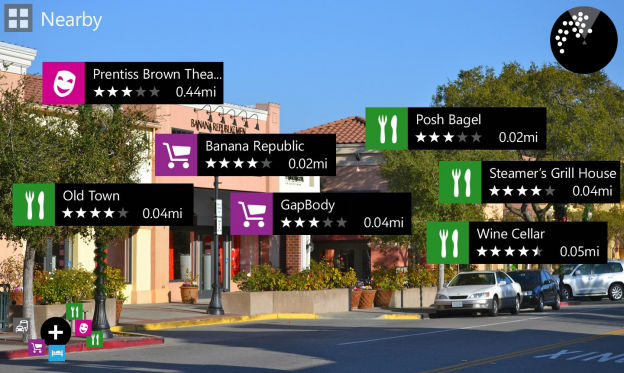
\includegraphics[width=15cm]{resources/nokia_city_lens-625x373-c.png}
\end{figure}




\label{def:hmd}
Muitas vezes, para exibição das informações, são usadas telas acopladas a capacetes,
chamadas \gls{HMD}. O \gls{HMD} consiste em um dispositivo acomodado na cabeça, de forma a cobrir os olhos.
Esses capacetes possuem uma tela onde são exibidas as imagens após seus processamentos pelo computador
responsável por criar a aplicação de Realidade Virtual ou de Realidade Aumentada. Também é possível
fornecer fones de ouvido ao usuário, para aumentar a imersão dele no mundo virtual gerado pelo sistema.
A Figura \ref{fig:hmd_example} mostra alguns tipos de \gls{HMD},

\begin{figure}[h!]
    \centering
    \caption{Exemplos de HDM (Head Mounted Display)}
    \label{fig:hmd_example}
    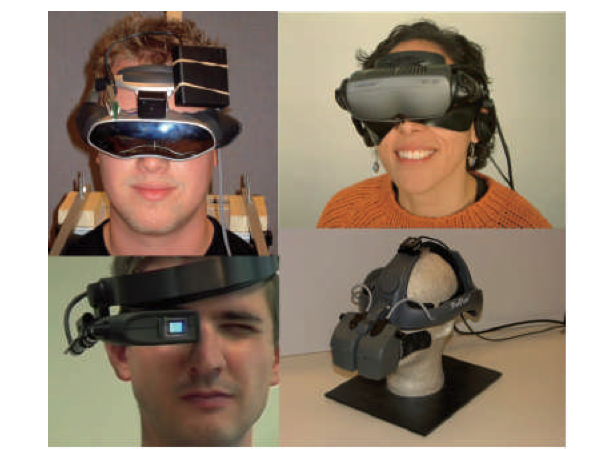
\includegraphics[width=13cm]{resources/HMD.png}
\end{figure}


Outra aplicação muito utilizada em Realidade Aumentada Móvel é o reconhecimento de códigos de barras e códigos QR
(\textit{QR Code}). Os códigos de barras comuns permitem detectar apenas dados numéricos, com o auxílio de um
leitor adequado (\textit{scanner}). Os Códigos QR (\textit{QR Code}, do inglês \textit{Quick Response}) podem 
representar dados alfanuméricos, permitindo descrever diversos outros tipos de dados, como número de telefone,
endereços de e-email e de \textit{web sites}, além de pequenos textos \cite{QRCodeSite}. A Figura 
\ref{fig:codigos-barras-qr-code} ilustra, do lado esquerdo, um código de barras comum e, do lado direito, um 
código QR.

\begin{figure}[h!]
    \centering
    \caption{Códigos de barras, usados em muitas aplicações de Realidade Aumentada Móvel}
    \label{fig:codigos-barras-qr-code}
    
\includegraphics[width=13cm]{resources/codigo-barras-qr-code.png}
\end{figure}


\cite{HandheldAR} escreveu uma dos mais completos trabalhos sobre Realidade Aumentada para
dispositivos móveis. Além de vários detalhes técnicos, como rastreamento de objetos sem marcadores 
(\textit{markless tracking}) em dispositivos móveis, diversos casos de uso são descritos, demonstrando
a aplicabilidade da Realidade Aumentada Móvel.



\section{Técnicas da Realidade Aumentada}

A Realidade Aumentada envolve sensores (como \gls{GPS} e bússola), visão computacional,
interação humano-computador, realidade virtual e muitas outras áreas do conhecimento.
As principais tecnologias da Realidade Aumentada incluem visualização (\textit{display}),
\textit{registration}, \textit{tracking} e interatividade \cite{ARFeatureMaching}.



\subsection{\textit{Tracking}}

O processo chamado de \textit{Tracking}, ou \textbf{rastreamento}, consiste na detecção da posição e da direção
do usuário. 


Em geral, sistemas de Realidade Aumentada projetados para uso externo baseiam-se em localização
utilizando \gls{GPS}, orientação magnética (bússola) e sensores de inércia para determinar a 
orientação do usuário no espaço tridimensional. 

De 1998 até 2008, a técnica de \textit{Tracking} foi o tema mais recorrente em pesquisas científicas
\cite{TrendsInAR}. Isso mostra como ela é essencial para o desenvolvimento e para o
aprimoramento das aplicações utilizando Realidade Aumentada.


Há três categorias de \textit{Tracking}: 1) \textit{Tracking} Baseada em Sensores,
2) \textit{Tracking} Baseada em Visão Computacional e 3) \textit{Tracking} Híbrida.

Além disso, existem duas formas principais de fazer rastreamento (\textit{tracking}): utilizando
marcadores e não os utilizando (\textit{markerless}). A primeira categoria é utilizada
predominantemente em rastreamento por visão computacional, enquanto a segunda está mais ligada
a rastreamento por sensores. Ambas essas técnicas serão discutidas com mais detalhes a seguir.




\subsubsection{Tracking Baseado em Sensores}

Esta técnica pode se basear em sensores magnéticos, acústicos, 
de inércia, óptico e mecânico. Todos eles possuem suas vantagens
e desvantagens. Por exemplo, sensores magnéticos possuem alta frequência de atualização,
mas são facilmente afetados por qualquer material metálico próximo que altere o campo 
magnético da região analisada. 

Essa categoria de \textit{Tracking} foi desenvolvida no final da década de 1990, e apresentada
no \textbf{IWAR}
\footnote{International Workshop on Augmented Reality} 
de 1998. Desde então, pesquisadores estão estudando maneiras de combinar diversos
sensores, a fim de obter resultados mais fiéis e confiáveis.


\subsubsection{Tracking Baseado em Visão Computacional}

Esta técnica utiliza processamento de imagens para calcular a posição do usuário no espaço. 
É a categoria de \textit{tracking} com mais pesquisas no \textbf{ISMAR}
\footnote{International Symposium on Mixed and Augmented Reality}, 
de 1998 a 2008, com mais
de 80\% de presença em artigos científicos publicados nesse simpósio.

Esse método é um dos mais conhecidos e usados em Visão Computacional, em se tratando de
\textit{tracking} com marcadores. Ele consiste em
colocar marcadores fixos no ambiente, reconhecê-los por meio de Visão Computacional, e,
por fim, calcular a posição e a direção da câmera, a partir dos resultados da etapa anterior.
A Figura \ref{fig:AR-marker} ilustra o processo de reconhecimento de marcadores nesta
técnica de rastreamento. A Figura \ref{fig:AR-marker-example1} apresenta um exemplo de aplicação
usando rastreamento (\textit{tracking}) baseado em marcadores.

\begin{figure}[h!]
    \centering
    \caption{Reconhecimento de marcadores no processo de rastreamento (\textit{tracking})}
    \label{fig:AR-marker}
    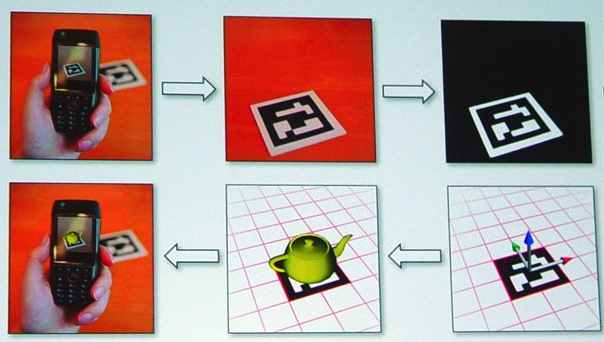
\includegraphics[width=15cm]{resources/marker-tracking.jpg}
\end{figure}



\begin{figure}[h!]
    \centering
    \caption{Exemplo de aplicação com rastreamento (\textit{tracking}) usando marcadores}
    \label{fig:AR-marker-example1}
    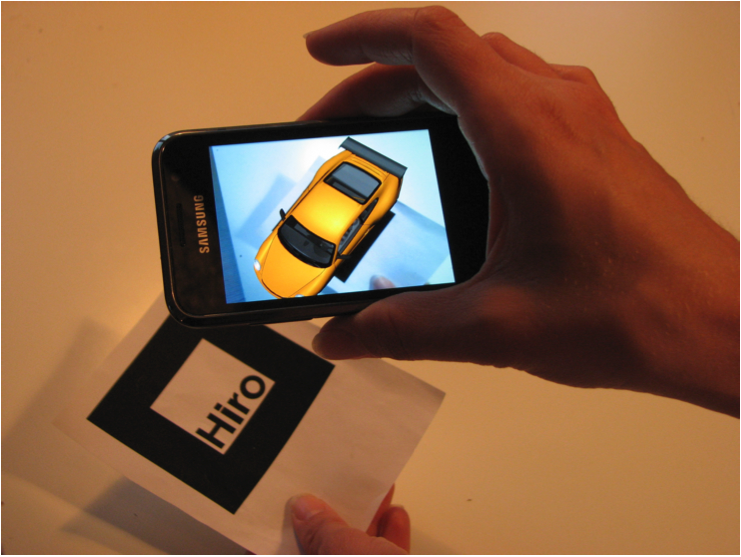
\includegraphics[width=15cm]{resources/marker-tracking-example1.png}
\end{figure}



\label{def:6dof}
Um dos conceitos explorados neste tipo de rastreamento é o \gls{6DOF},
que consiste na obtenção, por meio de sensores como acelerômetro e giroscópio, 
dos seis valores de posicionamento e orientação do dispositivo no espaço
tridimensional: três posições de rotação e três de translação. A Figura 
\ref{fig:6dof_data} mostra os seis dados relacionados com o \gls{6DOF}.

\begin{figure}[h!]
    \centering
    \caption{Os seis graus de liberdade (6DOF)}
    \label{fig:6dof_data}
    %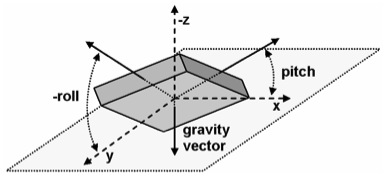
\includegraphics[width=15cm]{resources/6DOF.png}
    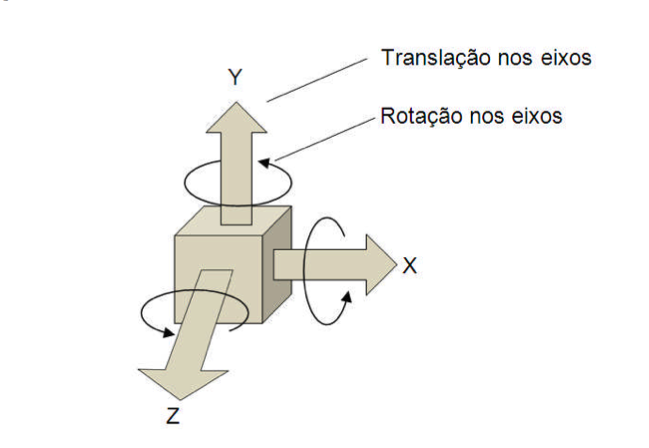
\includegraphics[width=15cm]{resources/6DoF-ptbr.png}
\end{figure}



O \textit{tracking} baseado em visão computacional busca associar traços de imagens 
digitais 2D em coordenadas no mundo real, em 3D.
A posição da câmera pode ser obtida projetando-se as coordenadas 3D nas coordenadas
da imagem 2D observada.    



\subsubsection{Tracking Híbrido}

Considerando que cada técnica citada anteriormente possui vantagens e desvantagens, 
foi proposta a combinação entre algumas delas. Por exemplo, Azuma\cite{SurveyAR}
propôs um sistema de Realidade Aumentada para uso externo que utiliza \gls{GPS}, 
sensores de inércia e visão computacional.

Em \cite{HybridTrackingOutdoorAR}, é abordado o desenvolvimento de um modelo de \textit{tracking}
híbrido, em que é utilizado um giroscópio (\textit{tracking} baseado em sensores)
e visão computacional.

O artigo \cite{HybridTrackingForGIS} também descreve uma técnica de \textit{tracking} híbrido,
em que são utilizadas informações de \gls{GPS} e de sensores de inércia para obter a localização,
a posição e a orientação do usuário no espaço.







\subsection{\textit{Registration}}

O processo chamado de \textit{Registration} consiste na sobreposição de objetos
virtuais às imagens da realidade. Esse método é fundamental para a garantia
de desempenho do sistema de Realidade Aumentada. Esse também é um dos principais
temas de pesquisa da Realidade Aumentada \cite{DevActuallyRegistration}.

O \textit{Registration} é um processo complexo, principalmente em aplicações de
Realidade Aumentada para uso externo (\textit{outdoor}). Ao se projetar um
sistema de Realidade Aumentada para uso externo, requisitos especiais de
equipamentos e de modelo de aplicação devem ser considerados. Em geral, eles
têm características de mobilidade, multi-dimensão e tempo real \cite{DevActuallyRegistration}.


O processo de \textit{Registration} também é crucial em muitas aplicações para uso interno
(\textit{indoor}). Imagine uma aplicação de Realidade Aumentada para uso médico, para biópsias.
Se o objeto virtual não estiver no local exato onde o verdadeiro tumor está, a agulha não atingirá
o local adequado e a biópsia falhará. Sem um processo de \textit{Registration} apurado e preciso, 
a Realidade Aumentada pode não ser aceitável em muitos tipos de aplicações, como a citada acima 
\cite{SurveyAR}.






Classifica-se o processo de \textit{Registration} em três grupos: 1) baseada em
rastreamento (\textit{tracker-based registration}), 2) baseada em conhecimento
(\textit{knowledge-based registration}) e 3) baseada em visão computacional
(\textit{computer vision-based registration}) \cite{DevActuallyRegistration}.



\subsubsection{Baseada em Rastreamento (\textit{Tracker-based Registration})}


O processo de \textit{Registration} baseado em rastreamento inclui: mecânica,
sensores magnéticos, GPS, ultrasonicos, inércia e óptica. A Tabela \ref{tab:track-reg-comp}
compara cada uma dessas técnicas.

\begin{table}[h!]
    \caption{Comparação entre técnicas de \textit{Registration}}
    \label{tab:track-reg-comp}
    \begin{tabular}{| p{5cm} | p{5cm} | p{5cm} |}
        \hline
        Tecnologia de \textit{Tracking} & Vantagens & Desvantagens \\
        \hline
        Mecânica & Exatidão, baixo atraso no processamento, sem influência visual ou magnética, fácil rastreamento de objetos pequenos & Uso limitado \\
        \hline
        Sensores Magnéticos & baixo preço, exatidão, sem interferências visuais, imune a sons, eficiente mesmo em áreas amplas & Facilmente influenciada por campos magnéticos e presença de metais no ambiente \\
        \hline
        GPS & ideal para áreas amplas & falta de precisão e atraso no processamento \\
        \hline
        Ultrasônico & baixo preço, sem influência de campos magnéticos, baixo uso de equipamentos & facilmente distorcida no ambiente, baixa precisão a grandes distâncias \\
        \hline
        Inércia & sem limitação de distâncias, alta velocidade, sem influência de visão ou campo magnético, tamanho pequeno e baixo custo & apenas 3 graus de liberdade\footnote{\textit{3 Degrees Of Freedom}: apenas 3 dos 6 possíveis graus de liberdade}, espalhamento e baixa precisão em altas velocidades \\
        \hline
    \end{tabular}
\end{table}




\subsubsection{Baseado em Conhecimento (\textit{Knowledge-based})}


O processo de \textit{Registration} Baseado em Conhecimento (\textit{Knowledge-based}) foi
proposto pelo Laboratório de Interface de Usuários, do Departamento de Ciência da Computação, 
da Universidade de Columbia, durante o desenvolvimento de um projeto de Realidade Aumentada.
Os rastreadores são fixados em equipamentos de formato conhecido, de forma a garantir a posição
e a orientação. O maior problema desse método é a necessidade de conhecer a estrutura dos equipamentos,
além de haver atraso e erros entre os rastreadores.



\subsubsection{Baseado em Visão Computacional (\textit{Computer vision-based})}

Devido à fácil teorização e à conveniência na realização, o \textit{registration} basedo em visão computacional
vem sendo a técnica de maior potencial em aplicações de Realidade Aumentada. Em teoria, ele possui alta precisão,
podendo chegar ao nível de \textit{pixels}.

O \textit{registration} baseado em visão computacional pode ser separado em duas categorias: 1) baseado em
calibragem de câmera (\textit{camera calibration}) e 2) baseado em transformação afim
(\textit{affine transformation}).

\begin{enumerate}
    \item \textbf{Baseado em Calibragem de Câmera}
    
    Esta é a categoria mais comum de \textit{registration} baseada em visão computacional. 
    Este método coloca marcadores no ambiente, reconhece-os por meio de visão computacional e, com essas informações, 
    calcula a posição e a orientação onde os objetos virtuais devem ser posicionados. 


    \item \textbf{Baseado em Transformação Afim}
    
    Esta técnica utiliza conceitos da Álgebra Linear para criar uma representação 2D de
    uma informação em 3D.
\end{enumerate}


\section{Realidade Aumentada \textit{Indoor} X \textit{Outdoor}}

Realidade Aumentada para ambientes internos (\textit{Indoor Augmented Reality})
geralmente utiliza \textit{tracking} baseada em marcadores, a fim de detectar
a direção para onde a câmera está apontando, ou mesmo qual objeto ela está
focalizando. Na Realidade Aumentada para ambientes externos (\textit{Outdoor Augmented Reality}),
é muito mais complexa a detecção da posição e da orientação do usuário. A utilização 
de marcadores torna-se muito mais complexa, devido ao tamanho da área abrangida pela aplicação.
Por isso, nesse tipo de Realidade Aumentada costuma-se usar \textit{tracking} baseado em sensores,
como \gls{GPS}, giroscópio e bússola, os quais permitem obter, com alta exatidão, a posição e a
orientação do usuário no espaço \cite{HybridTrackingForGIS}.





\section{Trabalhos Relacionados}
\label{sec:trab_relacionados}



Há diversos trabalhos relacionados a aplicações baseadas em Realidade
Aumentada \cite{MOOAR_Study}. 


Em \cite{HybridTrackingOutdoorAR}, é abordado o desenvolvimento de um modelo de \textit{tracking}
híbrido, em que é utilizado um giroscópio (\textit{tracking} baseado em sensores)
e visão computacional.


O artigo \cite{HybridTrackingForGIS} também descreve uma técnica de \textit{tracking} híbrido,
em que são utilizadas informações de \gls{GPS} e de sensores de inércia para obter a localização,
a posição e a orientação do usuário no espaço.


Um dos exemplos mais conhecidos atualmente é o \textit{Google Glass}
\footnote{\href{http://www.google.com/glass}{http://www.google.com/glass}}.
O Google Glass é um projeto do Google, com o objetivo de criar um óculos que exibe
informações para o usuário em \textit{displays} embutidos nas próprias lentes.

% No Museu de Ciência e Indústria (\textit{Museum of Science and Industry}), em Chicago,
% está exposta uma ferramenta de Realidade Aumentada que exibe, em uma mesa digital, a
% Tabela Periódica dos Elementos Químicos. Os usuários podem, arrastando um grupo de 
% elementos, criar simulações de reações químicas. A Figura \ref{fig:tabela-periodica-AR}
% ilustra essa ferramenta. O usuário pode arrastar dois ou mais elementos da Tabela
% Periódica para a área lateral direita da mesa, demarcada por uma circunferência, onde
% a simulação da reação ocorrerá.
% 
% 
% \begin{figure}[h!]
%     \centering
%     \caption{Aplicação de Realidade Aumentada do \textit{Museum of Science and Industry} para criar simulações de reações químicas}
%     \label{fig:tabela-periodica-AR}
%     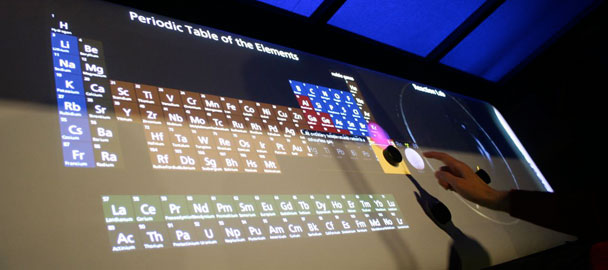
\includegraphics[width=14cm]{resources/tabela-periodica-AR.jpg}
% \end{figure}




Há, pelo menos, seis principais classes de aplicações de 
Realidade Aumentada exploradas até o momento: 1) médica, 2) manufatura e reparos,
3) anotações e visualização, 4) robótica, 5) entretenimento e 6) aplicações militares \cite{SurveyAR}.


\subsection{Área Médica}

Médicos podem utilizar a Realidade Aumentada como uma ferramenta de auxílio
no estudo e no treinamento para cirurgias e outros procedimentos. Várias 
aplicações estão explorando essa área. Na \textit{UNC Chapel Hill}, um grupo
de pesquisas coletou imagens do útero de mulheres grávidas usando ultrassonografia,
gerando uma representação 3D do feto dentro do útero e a exibindo em um \gls{HMD}, 
conforma a Figura \ref{fig:feto_utero_3d}. O objetivo é permitir ao médico analisar todos os movimentos
do feto dentro do útero, de forma que isso um dia torne-se uma espécie de estetoscópio 3D \cite{Feto3D}.

\begin{figure}[h!]
    \centering
    \caption{Imagem 3D de um feto dentro do útero (pesquisa da UNC Chapel Hill)}
    \label{fig:feto_utero_3d}
    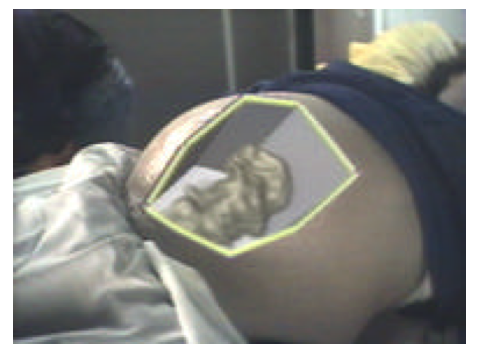
\includegraphics[width=10cm]{resources/feto-3d.png}
\end{figure}



\subsection{Manufatura e Reparos}

Outra aplicação para a Realidade Aumentada é na montagem, manutenção e reparo
de maquinários. Os procedimentos para essas atividades, em vez de estarem descritas
em texto na forma de manuais, poderia ser visualizada em 3D, sobrepostas aos
próprios equipamentos. É possível, inclusive, criar animações, mostrando exatamente
como proceder para realizar a tarefa. O grupo de Steve Feiner, em Columbia, desenvolveu
uma aplicação para manutenção de impressoras a \textit{laser} \cite{LaserPrinterAR}. 
A Figura \ref{fig:laser_printer_1} a visão externa a Figura \ref{fig:laser_printer_2} 
exibe a visão do usuário, onde uma 
imagem gerada por computador orienta o usuário a remover a bandeja de papel.


\begin{figure}[h!]
    \centering
    \caption{Visão externa do sistema de reparos de impressoras a laser}
    \label{fig:laser_printer_1}
    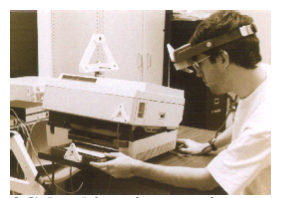
\includegraphics[width=10cm]{resources/laser-printer-1.png}
\end{figure}


\begin{figure}[h!]
    \centering
    \caption{Visão do usuário no sistema de reparos de impressoras a laser}
    \label{fig:laser_printer_2}
    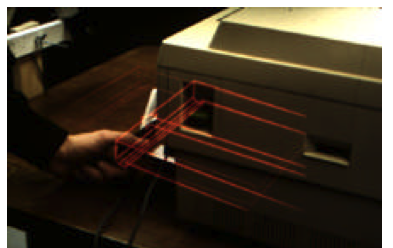
\includegraphics[width=10cm]{resources/laser-printer-2.png}
\end{figure}



\subsection{Anotação e Visualização}

Chang, W. \cite{MOOAR} propôs o
\textit{``Multi-Object Oriented Augmented Reality''} (MOOAR), também 
estudado por Chang and Tan em \cite{MOOAR_Study}. O \textit{MOOAR} foi
proposto para ambientes de aprendizado baseado em localização. Sua
implementação usa a Realidade Aumentada como principal ferramenta para
prover conteúdo interativo de aprendizado através de objetos virtuais.
O MOOAR visa a reduzir os desvios e aumentar a interação entre usuários,
objetos e conteúdo, a fim de melhorar a eficácia da aprendizagem.

Em \cite{AugmentedMaps} é proposta outra forma de Realidade Aumentada
baseada em mapas. Usando um mapa impresso como base, ao focar uma câmera sobre determinados
pontos do mapa, informações digitais eram sobrepostas à imagem, fornecendo maiores detalhes
ao usuário.



\subsection{Robótica}

Teleoperação de robôs é sempre uma tarefa complexa, especialmente quando o robô está distante, devido a falhas
na comunicação. Nessas condições, é preferível controlar um robô virtual, em vez do real. O operador planeja a 
rota do robô, guiando um robô virtual. Após traçado o trajeto, o robô real recebe as mesmas coordenadas recebidas
pelo virtual, o qual as segue, sem que haja erros ocasionados pela falha na comunicação entre o operador e o 
robô. Diversos autores criaram protótipos para essa finalidade \cite{RobotAR1,RobotAR2,RobotAR3}.


\subsection{Entretenimento}

A aplicação \textit{Archeoguide} \cite{Archeoguide} propôs uma viagem pelas ruínas de civilizações antigas usando
a Realidade Aumentada. O usuário visita a antiga Olympia, na Grécia, utilizando uma tela acoplada a um capacete
(\gls{HMD}), ligada a um computador semi-portátil, dentro de uma mochila. O sistema identifica 
artefatos e áreas danificadas, reconstruindo-as digitalmente na tela, e exibindo informações sobre os antigos 
esportes olímpicos. 

O projeto \textit{ALIVE}, do \textit{MIT Media Lab}, criou uma aplicação que adiciona ao ambiente
criaturas inteligentes virtuais, que reagem às ações dos usuários \cite{ArtificialLife}.





\subsection{Aplicações Militares}


A \textit{Boeing Computer Seattle} está desenvolvendo aplicações utilizando a Realidade Aumentada com o objetivo
de mostrar aos pilotos das aeronaves o maior número de informações relevantes sobre uma rota, ou mesmo auxiliá-los 
durante um combate. Já existem helicópteros que possuem um capacete para o piloto que está interligado com a mira 
de uma ou mais armas da aeronave. Dessa forma, para que o piloto mire o inimigo, basta olhar para ele \cite{ARCADE}.













\chapter{Aplicação Proposta}
\label{chapter:app_proposta}


As aplicações de geolocalização atualmente disponíveis na maioria dos dispositivos utilizam mapas ou imagens
provenientes de satélites. Para o usuário, esse tipo de visualização pode não ser satisfatória, pois não revela
informações e detalhes da realidade à sua volta.

Para o usuário de uma aplicação de geolocalização, o programa deveria não apenas exibir uma visão geral do terreno,
por meio de mapas ou imagens de satélite, mas, também, permitir visualizar informações de pontos de interesse ao
seu redor, bem como sua distância até eles, por meio de uma visualização do ambiente a partir de sua perspectiva. 
Ou seja, na tela de seu dispositivo, deveria ser exibida a imagem que ele vê com os próprios olhos, o que tornaria a
aplicação muito mais interativa.



Como trabalho prático, de implementação, foi desenvolvido um aplicativo
para dispositivos móveis usando técnicas de Realidade Aumentada para criar uma ferramenta
que facilite a localização de usuários nos campi da Universidade Federal do Paraná. 

O aplicativo fornece uma visualização de mapa, onde estão listados pontos de interesse
para alunos e funcionários da Universidade Federal do Paraná. Esse mapa será obtido por meio das
\glspl{API} oficiais do sistema operacional do dispositivo em que
o sistema é executado. As localizações de cada ponto de interesse são exibidas conforme
suas coordenadas geográficas (latitude e longitude).

Há outro modo de visualização, o qual envolve a Realidade Aumentada. Nesse modo,
a imagem da câmera é exibida na tela do dispositivo, com
os pontos de interesse próximos demarcados nela, de forma que, ao mover o aparelho
lateralmente, as referências aos pontos de interesse também se movem na tela, orientando o
usuário a como chegar a eles e informando qual é a distância até eles. Conforme o usuário
se move no espaço, atualizam-se os dados exibidos na tela. Isso inclui recalcular a
distância até os pontos de interesses, além de atualizar a visualização com essas novas
informações.

Foram mapeados alguns locais de interesse do campus Centro Politécnico,
da Universidade Federal do Paraná, em Curitiba, fixando pontos de referência, como, por exemplo:

\begin{itemize}
    \item Secretarias de cursos
    \item Coordenações de cursos
    \item Departamentos
    \item Restaurantes Universitários
    \item Centros Acadêmicos
    \item Lanchonetes
    \item Caixas Eletrônicos
    \item Bibliotecas
    \item Blocos de salas de aula
    \item Pontos de ônibus próximos aos campi
    \item Pontos do ônibus InterCampi
\end{itemize}



Há, também, uma interface de configurações, onde cada usuário pode adicionar, editar e remover
novos pontos de interesse que sejam úteis para ele.


A visualização em formato de mapas destaca os pontos de interesse por meio de alfinetes vermelhos,
que, quanto tocados, exibem o nome da localização. A Figura \ref{fig:pins-maps} ilustra a visualização de alguns
pontos do Centro Politécnico da Universidade Federal do Paraná, na visualização de mapas.

\begin{figure}{h!}
    \centering
    \caption{Exibição de locais na visualização de Mapas do Aplicativo Desenvolvido}
    \label{fig:pins-maps}
    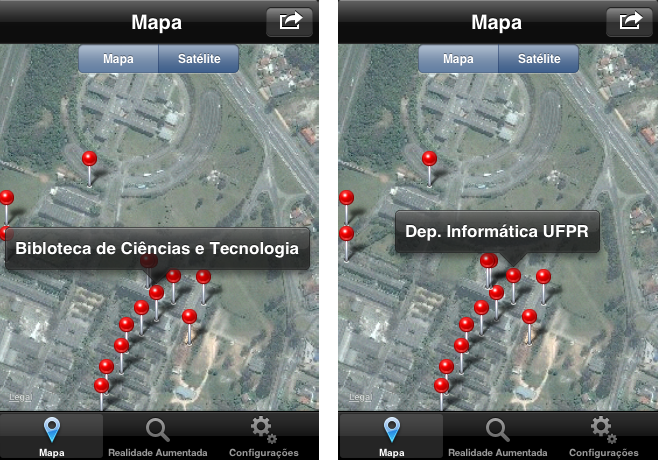
\includegraphics[width=14cm]{resources/App_Maps_Screenshots/mapa-pins.png}
\end{figure}

No canto superior esquerdo, há um botão que abre um menu de ações, ilustrado na 
Figura \ref{fig:maps-action-menu}. Por meio desse menu, é possível salvar a
atual localização do usuário, para criar um novo local de interesse; também é
possível centralizar o mapa na localização atual do usuário; além disso, também
é possível abrir uma lista dos locais salvos, para que o usuário selecione o ponto
que deseja visualizar no mapa.

\begin{figure}{h!}
    \centering
    \caption{Menu de ações relacionadas aos mapas no aplicativo desenvolvido}
    \label{fig:maps-action-menu}
    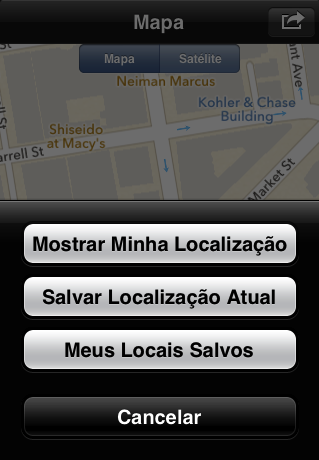
\includegraphics[width=10cm]{resources/App_Maps_Screenshots/action-menu.png}
\end{figure}



A Figura \ref{fig:App-AR-Screenshot} exibe um exemplo da visualização em Realidade Aumentada
do aplicativo.

\begin{figure}{h!}
    \centering
    \caption{Visualização em Realidade Aumentada do aplicativo proposto}
    \label{fig:App-AR-Screenshot}
    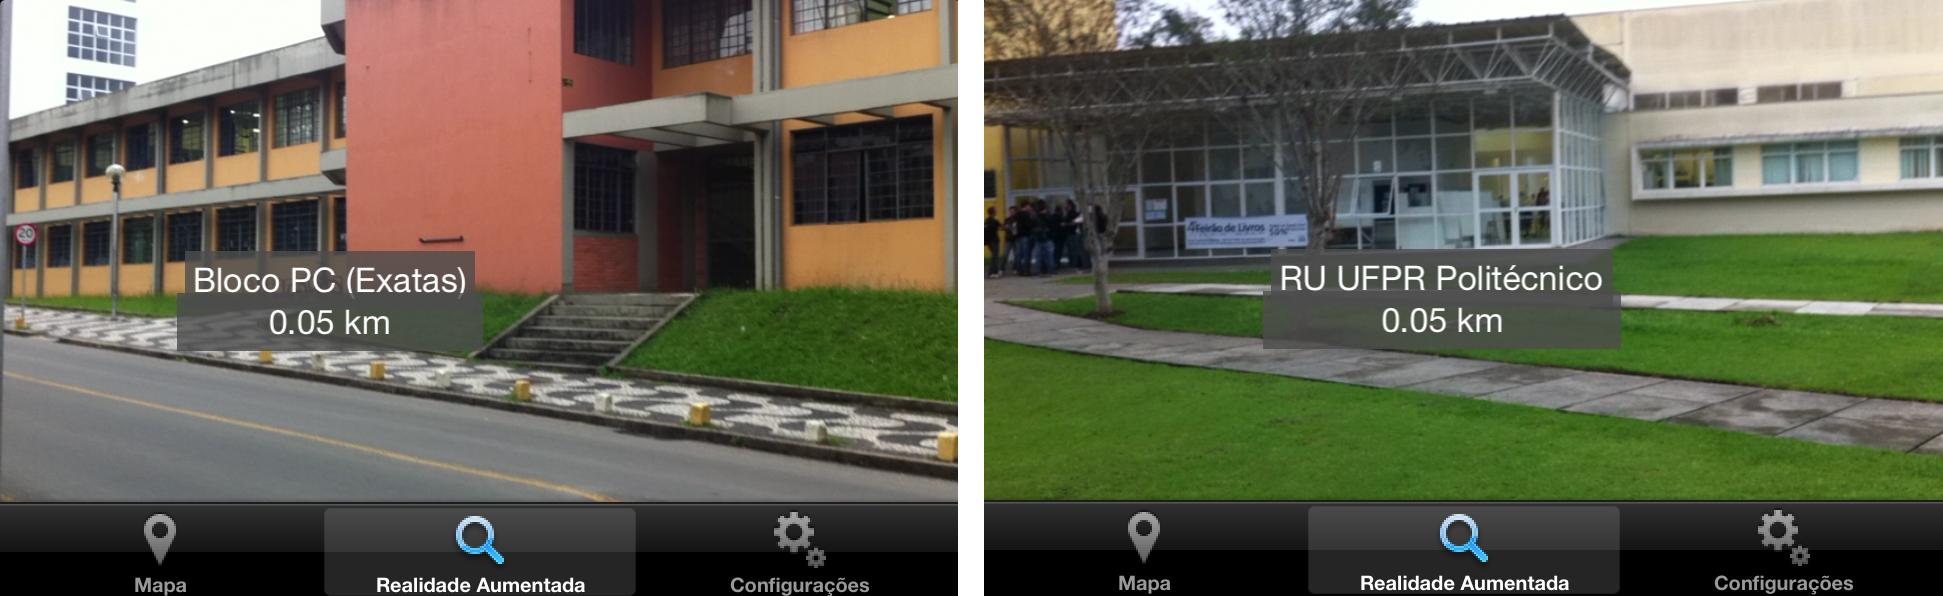
\includegraphics[width=17cm]{resources/App_AR_Screenshots/AR-sceenshot.png}
\end{figure}



\section{Detalhes da Implementação}


Como ferramenta base para o desenvolvimento, foi usado o \textbf{iPhone-AR-Toolkit}
\footnote{\href{https://github.com/nielswh/iPhone-AR-Toolkit}{https://github.com/nielswh/iPhone-AR-Toolkit}},
que também foi utilizado por William Chang e Qing Tan em \cite{MOOAR_Study}.
Essa ferramenta utiliza o conceito de \textit{``Multi-Object Oriented Augmented Reality''} (MOOAR), o qual 
foi descrito com mais detalhes na Seção \ref{sec:trab_relacionados} deste texto.

A aplicação utiliza técnicas de \textit{Tracking} e \textit{Registration} para utilização em ambientes 
externos (\textit{outdoor}). A detecção da posição e da orientação da câmera do dispositivo usado pelo 
usuário é feita utilizando-se
\gls{GPS}, acelerômetro e giroscópio. Ou seja, são utilizados \textit{Tracking} baseado em sensores 
(\textit{Sensor-Based Tracking}) e \textit{Registration} baseado em rastreamento 
(\textit{Tracking-based Registration}).


O dispositivo utilizado para testar a aplicação foi um Apple iPhone 4. A escolha foi feita devido à capacidade deste 
equipamento de obter dados de localização global (\gls{GPS}), além de possuir acelerômetro e giroscópio, permitindo
obter informações precisas da posição e da orientação do aparelho (\gls{6DOF}).


Com base na localização do usuário, a aplicação busca locais próximos conhecidos, cadastrados em uma base de dados
local do dispositivo, onde há, dentre outras informações, suas latitude e a longitude. Conforme a posição e a
orientação do usuário no espaço tridimensional, são exibidas imagens na tela do dispositivo, mostrando ao usuário
em qual direção cada local está e qual a distância até ele. A medida que o usuário se move, esses dados são atualizados,
de forma a funcionar como um guia para quem não conhece a região ou procura por um local ainda desconhecido para ele.

A linguagem utilizada foi a Objective-C, linguagem padrão da \gls{SDK} do iOS, sistema operacional para dispositivos 
móveis da Apple.


\subsection{Base de dados}

Para aplicações em dispositivos móveis de baixo consumo, costuma-se usar o SQLite
\footnote{\href{http://www.sqlite.org}{http://www.sqlite.org}} como \gls{SGBD}, 
por utilizar poucos recursos de armazenamento e processamento. A aplicação proposta
também utiliza o SQLite, por meio do \textit{Core Data}, uma interface fornecida 
pela Apple para acesso a bases de dados.

A estrutura do banco de dados é formada por apenas uma tabela, a qual armazena as
seguintes informações sobre os pontos de interesse: nome (uma \textit{string}), 
latitude (um número no formato \textit{float}) e longitude (um número no 
formato \textit{float}). A Figura \ref{fig:modelo_dados} mostra o modelo de dados 
da aplicação.


\begin{figure}[h!]
    \centering
    \caption{Modelo de dados da aplicação proposta}
    \label{fig:modelo_dados}
    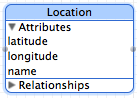
\includegraphics[width=4cm]{resources/App_Source_Code/db-scheme.png}
\end{figure}



O aplicativo é iniciado com uma base de dados inicial, com os principais pontos de interesse do campus Centro Politécnico
da Universidade Federal do Paraná. Essas informações iniciais ficam salvas em um arquivo \gls{XML}, formatado conforme
o padrão PLIST\footnote{\href{http://filext.com/file-extension/PLIST}{http://filext.com/file-extension/PLIST}} 
(\textit{Property List}), com os dados dos pontos de interesse, como nome, latitude e longitude. A Figura 
\ref{fig:plist-file} mostra como é a estrutura desse arquivo. O Algoritmo \ref{alg:load-plist-file} exibe o
trecho de código que carrega os dados desse arquivo e os salva na base de dados.


\begin{figure}[h!]
    \centering
    \caption{Arquivo XML com os dados iniciais da base de dados da aplicação proposta}
    \label{fig:plist-file}
    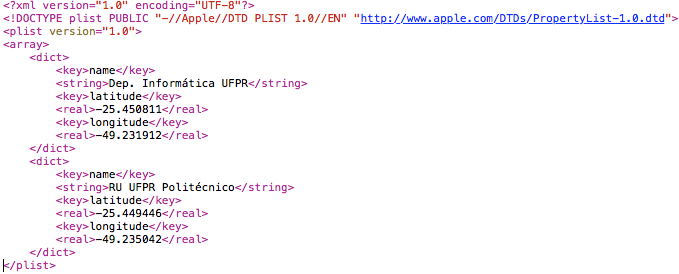
\includegraphics[width=17cm]{resources/App_Source_Code/plist-file.png}
\end{figure}



\begin{sourcecode}{alg:load-plist-file}{Trecho de código que carrega os dados do Arquivo XML para o SQLite}
- (void) loadInitialCoreDataInfo
{
    // array com os arquivos PLIST que devem ser carregados no Core Data
    NSArray *plistFiles = @[@{@"basename" : @"places_politecnico", @"extension" : @"plist"}];

    for ( NSDictionary *plistDict in plistFiles )
    {
        NSString *path = [[NSBundle mainBundle] pathForResource:plistDict[@"basename"] ofType:plistDict[@"extension"]];

        NSFileManager *fileManager = [NSFileManager defaultManager];

        if ( ! [fileManager fileExistsAtPath:path] )
        {
            NSLog(@"Arquivo '%@' nao existe", path);
            continue;
        }

        NSArray *locations = [NSArray arrayWithContentsOfFile:path];

        for ( NSDictionary *locationDict in locations )
        {
            NSString *name = locationDict[@"name"];
            NSNumber *latitude = locationDict[@"latitude"];
            NSNumber *longitude = locationDict[@"longitude"];

            [Location saveLocation:name latitude:[latitude floatValue] longitude:[longitude floatValue]];
        }
    }
}
\end{sourcecode}


\subsection{Integração com o iPhone-AR-Toolkit}

O \textit{iPhone-AR-Toolkit} não é uma biblioteca, nem um \textit{framework}. Ele é um
projeto ainda em desenvolvimento, com alguns recursos não muito aprimorado até o momento. Ou seja,
não basta apenas importar os arquivos e chamar um método específico. Porém, sua integração
com outras aplicações não é muito complexa. Seguindo o padrão da aplicação de demonstração, 
disponibilizada também no \textit{GitHub}, com algumas modificações e adaptações, é 
possível ter uma aplicação funcional.

A \gls{SDK} do iOS utiliza o padrão de projeto \textit{Delegation}. Esse é um padrão
utilizado na Programação Orientada a Objetos onde um objeto A, em vez de executar uma
determinada tarefa, delega-a para um objeto B. O \textit{iPhone-AR-Toolkit} também
utiliza esse padrão de projeto em diversas partes de seu código.


O Algoritmo \ref{alg:display_ar} ilustra o método responsável por carregar a \textit{view}
da Realidade Aumentada. O objeto \texttt{arc} é uma instância da classe 
\texttt{AugmentedRealityController}, que é responsável pelas operações relacionadas à
Realidade Aumentada. O objeto \texttt{arView} é uma instância da classe \texttt{UIView},
padrão da \gls{SDK} do iOS. Durante a instanciação de \texttt{arc}, na linha 5, é definido o seu
\textit{delegate} para \textit{self}, ou seja, o próprio objeto. Nesse ponto é usado o 
padrão \textit{Delegation}, quando a classe atual é responsável por executar tarefas da
\texttt{AugmentedRealityController}.


\begin{sourcecode}{alg:display_ar}{Método responsável pelo carregamento da \textit{view} de Realidade Aumentada}
- (void) displayAR
{
    if ([ARKit deviceSupportsAR])
    {
        arc = [[AugmentedRealityController alloc] initWithView:[self arView] parentViewController:self withDelgate:self];

        [self populateGeoLocations];
    }
    else
    {
        [self notSupportView];
    }
}
\end{sourcecode}


Antes de habilitar a funcionalidade de Realidade Aumentada, é necessário verificar se o dispositivo
suportará esse recurso. Para isso, o equipamento deve possuir câmera, além de sensor de \gls{GPS},
para detecção da localização do usuário. O Algoritmo \ref{alg:device-supports-ar} mostra o método
responsável por essas verificações. Para detecção da presença de câmera, usam-se algumas classes e
métodos do \textit{framework} \texttt{AVFoundation}, nativo do iOS. Para verificação da presença de
\gls{GPS} e suporte a localização, usa-se o método \texttt{headingAvailable])}, da classe 
\texttt{CLLocationManager}, presente no \textit{framework} \texttt{CoreLocation}, 
também nativo do iOS.

\begin{sourcecode}{alg:device-supports-ar}{Método para verificar se o dispositivo suporta o recurso de Realidade Aumentada}
+(BOOL)deviceSupportsAR
{
    // verifica o suporte a captura de video
    NSArray *devices = [AVCaptureDevice devices];

    BOOL suportsVideo = NO;

    if (devices != nil && [devices count] > 0) 
    {
        for (AVCaptureDevice *device in devices) 
        {
            if ([device hasMediaType:AVMediaTypeVideo]) 
            {
                suportsVideo = YES;
                break;
            }
        }
    }

    if (!suportsVideo)
    {
        return NO;
    }
    
    // verifica suporte a GPS
	if ( [CLLocationManager headingAvailable])
	{
		return NO;
	}

	return YES;
}
\end{sourcecode}



O método \texttt{populateGeoLocations} é responsável por buscar na base de dados as informações
acerca dos pontos de interesse, como nome, latitude e longitude. Esse método também cria as 
\textit{views} que servirão de marcadores, as quais serão sobrepostas às imagens da câmera, 
conforme a localização e a direção do dispositivo. O Algoritmo \ref{alg:populate-geolocations}
exibe a implementação desse método.



\begin{sourcecode}{alg:populate-geolocations}{Método responsável pelo carregamento das localizações e criação dos marcadores na tela do dispositivo}
- (void) populateGeoLocations
{
    GEOLocations* locations = [[GEOLocations alloc] initWithDelegate:self];

    if ([[locations returnLocations] count] > 0)
    {
        for (ARGeoCoordinate *coordinate in [locations returnLocations])
        {

            MarkerView *cv = [[MarkerView alloc] initForCoordinate:coordinate withDelgate:self] ;
            [coordinate setDisplayView:cv];

            [arc addCoordinate:coordinate];
        }
    }
}
\end{sourcecode}



O método \texttt{initWithView:parentViewController:withDelgate:}, utilizado na linha 5 do
Algoritmo \ref{alg:display_ar}, é responsável por inicializar o objeto 
\texttt{AugmentedRealityController}, subclasse de \texttt{NSObject}, a qual é a classe base
de todos os objetos no Objective-C. Além de definir algumas propriedades internas do objeto, 
este método instancia os objetos responsáveis por carregar as imagens provenientes da câmera
do dispositivo. Note que esse procedimento é realizado dentro de um \texttt{if}, na linha 22, o qual verifica
se a aplicação não estará sendo executada no \textit{iPhone Simulator}, simulador do iPhone disponibilizado
pela Apple juntamente com a \gls{SDK} do iOS. Como o simulador não possui câmera, essa verificação é
necessária, para evitar erros durante a execução. O método também adiciona, na linha 61, um método responsável por
redesenhar a \textit{view} se a orientação do dispositivo mudar (vertical ou horizontal). Para isso, é usada
a class \texttt{NSNotificationCenter}, do iOS, que registra notificações que ficam disponíveis durante todo o 
tempo de vida da aplicação.


\begin{sourcecode}{alg:initAR}{Método responsável por instanciar a \textit{view} de Realidade Aumentada e iniciar os recursos de câmera e GPS}
- (id)initWithView:(UIView*)arView parentViewController:(UIViewController*)parentVC withDelgate:(id<ARDelegate>) aDelegate
{    
    if (!(self = [super init]))
		return nil;

    [self setParentViewController:parentVC];
    [self setDelegate:aDelegate];

    latestHeading   = HEADING_NOT_SET;
    prevHeading     = HEADING_NOT_SET;

    [self setMaximumScaleDistance: 0.0];
	[self setMinimumScaleFactor: SCALE_FACTOR];
	[self setScaleViewsBasedOnDistance: NO];
	[self setRotateViewsBasedOnPerspective: NO];
	[self setMaximumRotationAngle: M_PI / 6.0];
    [self setCoordinates:[NSMutableArray array]];
    [self currentDeviceOrientation];

	degreeRange = [arView frame].size.width / ADJUST_BY;

#if !TARGET_IPHONE_SIMULATOR

    NSError *error = nil;
    AVCaptureSession *avCaptureSession = [[AVCaptureSession alloc] init];
    AVCaptureDevice *videoCaptureDevice = [AVCaptureDevice defaultDeviceWithMediaType:AVMediaTypeVideo];
    AVCaptureDeviceInput *videoInput = [AVCaptureDeviceInput deviceInputWithDevice:videoCaptureDevice error:&error];

    if (videoInput) {
        [avCaptureSession addInput:videoInput];
    }
    else {
        // Handle the failure.
    }

    AVCaptureVideoPreviewLayer *newCaptureVideoPreviewLayer = [[AVCaptureVideoPreviewLayer alloc] initWithSession:avCaptureSession];

    [[arView layer] setMasksToBounds:YES];
    [newCaptureVideoPreviewLayer setFrame:[arView bounds]];
    [newCaptureVideoPreviewLayer setVideoGravity:AVLayerVideoGravityResizeAspectFill];

    if ([[newCaptureVideoPreviewLayer connection] isVideoOrientationSupported])
        [[newCaptureVideoPreviewLayer connection] setVideoOrientation:cameraOrientation];

    [newCaptureVideoPreviewLayer setVideoGravity:AVLayerVideoGravityResizeAspectFill];
    [[arView layer] insertSublayer:newCaptureVideoPreviewLayer below:[[[arView layer] sublayers] objectAtIndex:0]];

    [self setPreviewLayer:newCaptureVideoPreviewLayer];

    [avCaptureSession setSessionPreset:AVCaptureSessionPresetHigh];
    [avCaptureSession startRunning];

    [self setCaptureSession:avCaptureSession];  

#endif

    CLLocation *newCenter = [[CLLocation alloc] init];

	[self setCenterLocation: newCenter];

	[[NSNotificationCenter defaultCenter] 
	 addObserver:self 
	 selector:@selector(deviceOrientationDidChange:)
     name:UIDeviceOrientationDidChangeNotification 
     object:nil];

	[self startListening];
    [self setDisplayView:arView];

  	return self;
}
\end{sourcecode}


O método \texttt{startListening}, na linha 66 do Algoritmo \ref{alg:initAR},
é encarregado de iniciar a atualização da localização, conforme o usuário
se move no espaço, além de habilitar o uso do acelerômetro, para detecção
da orientação do dispositivo. O Algoritmo \ref{alg:startListening} mostra a 
implementação desse método.

\begin{sourcecode}{alg:startListening}{Implementação do método \texttt{startListening}}
- (void)startListening
{
	// start our heading readings and our accelerometer readings.
	if (![self locationManager]) {
		CLLocationManager *newLocationManager = [[CLLocationManager alloc] init];

        [newLocationManager setHeadingFilter: HEADING_FILTER];
        [newLocationManager setDistanceFilter:DISTANCE_FILTER];
		[newLocationManager setDesiredAccuracy: kCLLocationAccuracyNearestTenMeters];
		[newLocationManager startUpdatingHeading];
		[newLocationManager startUpdatingLocation];
		[newLocationManager setDelegate: self];

        [self setLocationManager: newLocationManager];
	}

	if (![self accelerometerManager]) {
		[self setAccelerometerManager: [UIAccelerometer sharedAccelerometer]];
		[[self accelerometerManager] setUpdateInterval: INTERVAL_UPDATE];
		[[self accelerometerManager] setDelegate: self];
	}

	if (![self centerCoordinate]) 
		[self setCenterCoordinate:[ARCoordinate coordinateWithRadialDistance:1.0 inclination:0 azimuth:0]];
}
\end{sourcecode}


O método \texttt{updateLocations}, cuja implementação está exibida no Algoritmo
\ref{alg:updateLocations}, é o responsável por alterar os marcadores de pontos de
interesse exibidos na tela do dispositivo, conforme o usuário se move.

\begin{sourcecode}{alg:updateLocations}{Implementação do método \texttt{updateLocations}}
- (void)updateLocations
{
	for (ARGeoCoordinate *item in [self coordinates]) {

        UIView *markerView = [item displayView];

		if ([self shouldDisplayCoordinate:item]) {

            CGPoint loc = [self pointForCoordinate:item];
            CGFloat scaleFactor = SCALE_FACTOR;

			if ([self scaleViewsBasedOnDistance]) 
				scaleFactor = scaleFactor - [self minimumScaleFactor]*([item radialDistance] / [self maximumScaleDistance]);

			float width	 = [markerView bounds].size.width  * scaleFactor;
			float height = [markerView bounds].size.height * scaleFactor;

			[markerView setFrame:CGRectMake(loc.x - width / 2.0, loc.y, width, height)];
            [markerView setNeedsDisplay];

			CATransform3D transform = CATransform3DIdentity;

			// Set the scale if it needs it. Scale the perspective transform if we have one.
			if ([self scaleViewsBasedOnDistance]) 
				transform = CATransform3DScale(transform, scaleFactor, scaleFactor, scaleFactor);

			if ([self rotateViewsBasedOnPerspective]) {
				transform.m34 = 1.0 / 300.0;
			}
			[[markerView layer] setTransform:transform];

			//if marker is not already set then insert it
			if (!([markerView superview])) {
				[[self displayView] insertSubview:markerView atIndex:1];
			}
		} 
		else 
            if ([markerView superview])
                [markerView removeFromSuperview];

	}
}
\end{sourcecode}









\chapter{Conclusão}
\label{chapter:conclusao}


Nota-se que a Realidade Aumentada é um tema que vem ganhando muito espaço
nos últimos 20 anos, principalmente em pesquisa acerca 
de técnicas de \textit{Tracking} e \textit{Registration} \cite{TrendsInAR}.
Existem diversas aplicações para a Realidade Aumentada, principalmente para
aprendizado e reconhecimento de ambientes. Embora ela venha crescendo lentamente,
cada vez mais pesquisadores se
interessam por sua evolução.

Com o avanço das tecnologias móveis, dos \textit{smartphone} e \textit{tablets}, 
a área de Realidade Aumentada Móvel deve crescer ainda mais, abrindo espaço para
novas categorias de aplicações, que auxiliarão os usuários nas tarefas do
dia-a-dia, como o \textit{Google Glass}, citado na Seção \ref{sec:trab_relacionados}.


Entre 1998 e 2007, de 100 artigos de Realidade Aumentada avaliados por \cite{TrendsInAR},
um total de 63 estudavam as técnicas de \textit{Tracking} e \textit{Registration}. Essas
áreas merecem atenção especial, por se tratarem de técnicas essenciais para o desenvolvimento
da Realidade Aumentada.


\section{Conclusões Acerca da Aplicação Desenvolvida}

O \textit{iPhone-AR-Toolkit} é uma ferramenta ainda em desenvolvimento e de integração não muito 
fácil com outras aplicações. Porém, vem recebendo diversas contribuições e, em um futuro próximo,
deve se tornar uma biblioteca de fácil implementações em aplicações de Realidade Aumentada. 

Um dos pontos fracos dessa ferramenta é a falta de integração com camadas de dados. Todas as 
informações de latitude e longitude estavam presentes dentro do código-fonte. Foi necessário
criar uma camada de dados e modificar a ferramenta para integrar-se com ela.

Outra falha aparente é a detecção da posição exata do usuário. Essa falha está relacionada com a precisão
do \gls{GPS}. Não se pode afirmar ao certo se é um problema da ferramenta ou do dispositivo usado. São 
necessários mais testes, em diferentes plataformas e localizações, para chegar a essa conclusão.

De modo geral, o \textit{iPhone-AR-Toolkit} mostrou-se estável e confiável para a aplicação proposta.



\section{Outras Possíveis Aplicações}

Esse tipo de aplicação permite explorar diversas outras áreas de interesse.
É possível usar a mesma técnica descrita aqui para guiar usuários em ambientes
turísticos, como museus, onde são exibidas na tela direções para pontos de interesse,
além das informações relacionadas a eles.

Também é possível adaptar essa técnica em sistemas de \gls{GPS} utilizados em veículos,
permitindo, além da visão aérea do mapa, uma visão da mesma perspectiva do usuário, onde 
o dispositivo orienta o usuário para qual direção ele deve ir a fim de chegar em seu destino.

Uma possibilidade muito interessante é no ramo de aplicações assistivas. Em vez de exibir na tela
locais conhecidos e suas direções até eles, o programa poderia orientar usuários cegos, por meio de
áudio, a fim de guiá-los em direção de seus destinos. 




%====================================


% ----------------------------------------------------------
% Referências bibliográficas
% ----------------------------------------------------------
\bibliography{tg2}



\end{document}
